\chapter{The Π-Ware library}
\label{chap:piware}

    Π-Ware is an \ac{EHDL} that allows for circuit description (modelling),
    simulation, reasoning (proving correctness or other properties), and synthesis to netlists.
    In this chapter we will describe in detail how the Π-Ware library is organized,
    what principles are behind some of the most important design decisions taken in its development,
    and how to use Π-Ware to model, simulate and reason about circuit behaviour.

    The reader is assumed to be familiar with the \emph{Agda} programming language,
    as this is the language in which Π-Ware is embedded.
    An introductory-level knowledge of dependent type theory in general is also appreciated.


    \section{Circuit Syntax}
    \label{sec:circuit-syntax}
        %% Shallow vs. deep embedding
        %% Structural modelling
        %%     Represent connections among circuits in the DSL, \emph{not in the metalanguage}
        %%     Avoid having to deal with observable sharing

        The most basic activity allowed by Π-Ware is the \emph{description} of circuits:
        as already mentioned briefly in the introduction, Π-Ware is \emph{deeply} embedded,
        which means there is a \emph{datatype} whose values are circuits.

        A deep embedding was chosen in order to allow for semantics other than execution (simulation).
        Particularly, the possibility of \emph{synthesizing} circuit models was a requirement
        kept in mind throughout the whole development.

        The circuit datatype (\AD{ℂ'}) is the most \emph{fundamental} of the whole library.
        It is defined as an dependent inductive family, indexed by two natural numbers,
        as shown in Listing~\ref{lst:Circuit-core}.

        \begin{listing}[h]
            \ExecuteMetaData[agda/latex/PiWare/Circuit/Core.tex]{Circuit-core}
            \caption{The core circuit type (\AD{ℂ'}) of Π-Ware. \label{lst:Circuit-core}}
        \end{listing}

        A \emph{structural representation} of a circuit is achieved by the constructors of \AD{ℂ'}.
        This is in stark contrast with the the description style used in the Lava family, for example.
        In Lava, the constructors of the circuit datatype represent solely logic (or arithmetic) gates,
        and metalanguage (Haskell) constructs such as application, tupling and local naming are
        used to represent sequencing, parallel composition, loops and sharing.
        In Π-Ware, on the other hand, explicit constructors represent these combinations,
        avoiding the need to implement some form of \emph{observable sharing}~\cite{gill-typesafe-observable-sharing}.

        The indices of \AD{ℂ'} represent, respectively, the \emph{size} of the circuit's input and output.
        This can be thought of as the number of "wires" entering (resp. leaving) that circuit.
        Notice that the representation of inputs and outputs used in \AD{ℂ'} is untyped and unstructured.
        However, there is another -- higher-level -- circuit datatype (\AD{ℂ}),
        which adds a layer of typing \emph{on top} of \AD{ℂ'},
        and constitutes the actual intended "interface" between the user (hardware designer) and Π-Ware.
        This abstraction layer will be discussed in more detail on Section~\ref{subsec:high-level-circuit}.

        To better understand the reasoning behind the design of the low-level \AD{ℂ'} datatype,
        its constructors can be considered to belong to one of three categories:

        \begin{description}
            \item[Fundamental:] These construct "predefined", or "atomic" circuits, with no sub-components.
                \begin{itemize}
                    \item \AI{Nil}: The \emph{empty circuit}. Performs no computation and has neither inputs nor outputs.
                        It is mainly useful as a "base case" when building large circuits with recursive definitions.
                    \item \AI{Gate}: Constructs a chosen circuit among those provided by a \emph{gate library}
                        passed as parameter to the \AM{Circuit} module.
                    \item \AI{Plug}: Constructs a "rewiring" circuit. Performs no computation,
                        but can be used to apply permutations, associativity and to duplicate or discard wires.
                \end{itemize}
            \item[Structural:] Represent ways in which smaller circuits can be interconnected to build a bigger one.
                \begin{itemize}
                    \item \AI{c₁ ⟫' c₂}: Sequential composition.
                        Given $c₁$ and $c₂$, connects the output of $c₁$ into the input of $c₂$.
                    \item \AI{c₁ |' c₂}: Parallel composition.
                        Splits the input into two parts, connected to $c₁$ and $c₂$,
                        and rejoins the outputs of $c₁$ and $c₂$ into a single output.
                    \item \AI{c₁ |+' c₂}: Tagged branching.
                        Based on the value of a \emph{tag} given in one of the input wires,
                        feed the remaining input wires into \emph{either} $c₁$ or $c₂$.
                \end{itemize}
            \item[Delay:]
                The \AI{DelayLoop} constructor belongs to a category of its own.
                Its purpose is to construct a state-holding circuit given a purely combinational circuit as argument.
        \end{description}

        These descriptions are just a rough summary of the \emph{synthesis semantics} of Π-Ware, that is,
        how each circuit constructor creates a netlist, given netlists as arguments.
        The precise \emph{definitions} of the synthesis semantics is given in Section~\ref{sec:circuit-semantics}.
        The same section also contains a detailed definition and explanation of a simulation semantics
        for Π-Ware circuits, both purely combinational and sequential ones.

        \subsection{Design discipline enforced by circuit constructors}
            The several constructors of \AD{ℂ'} "calculate" the port sizes of the circuits they construct,
            based on the sizes of the circuits given as arguments.
            These calculations implement \emph{structural well-formedness} rules for circuits.
            One example of such rule can be seen in the case of parallel composition:

            \begin{center}
                \begin{code}
                    \>[4]\AgdaInductiveConstructor{\_|'\_} \<[11]%
                    \>[11]\AgdaSymbol{:} \AgdaSymbol{∀} \AgdaSymbol{\{}\AgdaBound{i₁} \AgdaBound{o₁} \AgdaBound{i₂} \AgdaBound{o₂}\AgdaSymbol{\}} \<[30]%
                    \>[30]\AgdaSymbol{→} \AgdaDatatype{ℂ'} \AgdaBound{i₁} \AgdaBound{o₁} \AgdaSymbol{→} \AgdaDatatype{ℂ'} \AgdaBound{i₂} \AgdaBound{o₂} \AgdaSymbol{→} \AgdaDatatype{ℂ'} \AgdaSymbol{(}\AgdaBound{i₁} \AgdaPrimitive{+} \AgdaBound{i₂}\AgdaSymbol{)} \AgdaSymbol{(}\AgdaBound{o₁} \AgdaPrimitive{+} \AgdaBound{o₂}\AgdaSymbol{)}\<%
                \end{code}
            \end{center}

            In this case, the input (resp. output) size of the composed circuit equals the \emph{sum}
            of the input (resp. output) sizes of the constituent sub-circuits.
            Other such rules are also imposed by \AI{\_⟫'\_}, \AI{\_|+'\_} and \AI{Plug}.
            Together, all of them ensure:

            \begin{description}
                \item[No floating wires] Circuit sizes need to match in order for the usage of a constructor
                    to be type-correct. In particular, no circuit \emph{input} wires are ever left "disconnected".
                    Figure~\ref{fig:sequencing-floating} illustrates an example of a situation banned by the sizing rule present
                    in the type of \AI{\_⟫'\_}.

                    \begin{figure}[h]
                        \centering{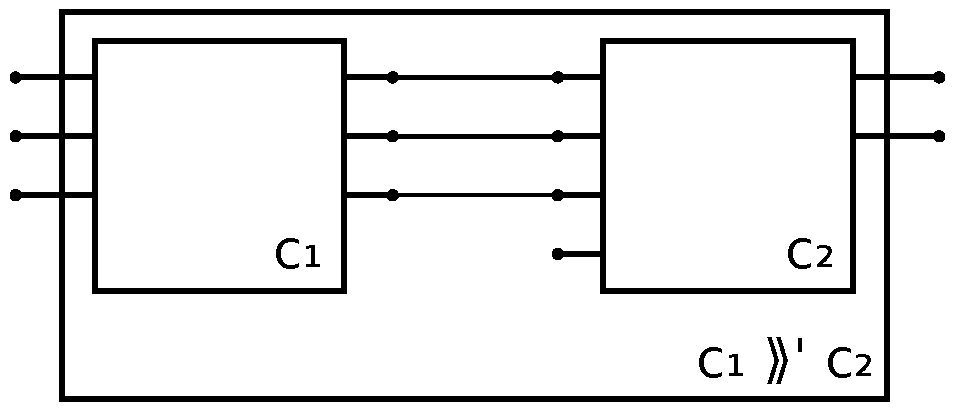
\includegraphics[width=0.6\textwidth]{imgs/sequencing-floating.pdf}}
                        \caption{Example of circuit banned by the type of \AI{\_⟫'\_}.\label{fig:sequencing-floating}}
                    \end{figure}

                \item [No short-circuits] The \AI{Plug} constructor, the only one which can be used for
                    "rewiring" purposes, has a type which forbids connecting multiple sources to the same load.
                    Its argument is a \emph{function from outputs to inputs}.
                    In this way, definitions connecting multiple inputs to the same output are banned,
                    as they are \emph{not} functions from outputs to inputs.
                    Also, when a plug is used between two sub-circuits $c₁$ and $c₂$,
                    a definition in which an \emph{input} of $c₂$ would be left "disconnected" is disallowed by Agda,
                    as such a definition would not be \emph{total}.
                    The diagram on Figure~\ref{fig:plug-seq-disconnected-input} represents such a banned situation:

                    \begin{figure}[h]
                        \centering{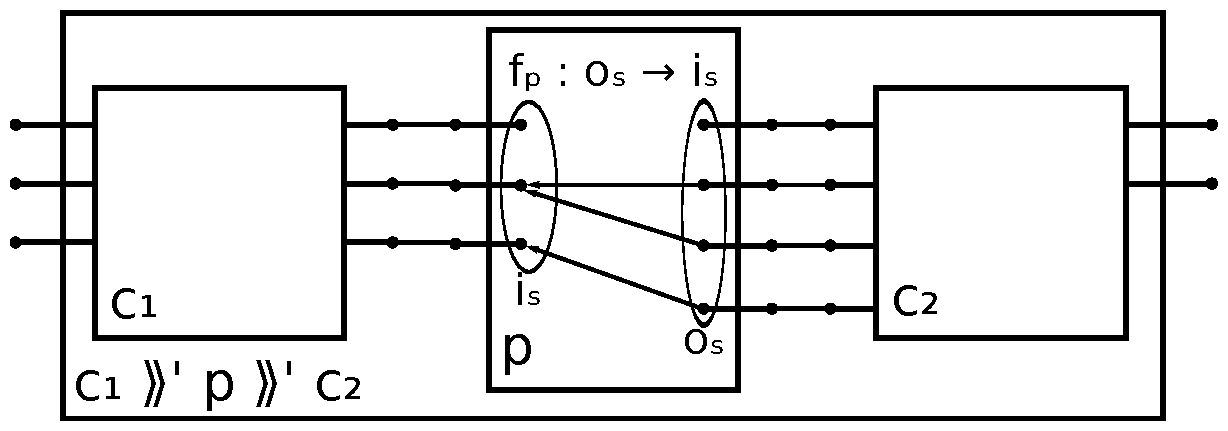
\includegraphics[width=0.8\textwidth]{imgs/plug-seq-disconnected-input.pdf}}
                        \caption{This circuit cannot be constructed because $f_{p}$ is not \emph{total}.\label{fig:plug-seq-disconnected-input}}
                    \end{figure}
            \end{description}

            %% TODO: explain Plug more?


    \section{Abstraction Mechanisms}
    \label{sec:circuit-abstraction}
        Several of the definitions (modules, datatypes, functions) of Π-Ware are parameterized
        in order to provide for better code reuse.
        The library allows for a choice of the type of data carried in individual wires,
        the types that serve as inputs and ouputs to circuits,
        and the set of fundamental gates from which circuits are built.

        In this section we present how this flexibility is achieved,
        which requirements are imposed upon the parameters in each case of parameterization.
        Also, the motivation behind the chosen requirements is presented,
        based on the general goals of Π-Ware as well as the wish to impose as few constraints as possible.

        %% Data abstraction (atom vectors x arbitrary synthesizable types)
        %%     Atom (enumeration axioms)
        %%     Word / Synthesizable
        %%         Proof search?
        %% Gate abstraction (Technology primitives x Semantic fundamentals)
        %%     Circuits descriptions are parameterized by a set of fundamental gates
        %%         Always combinational
        %%         Their correctness is assumed
        %%     For synthesis, still need to give these gates a description in terms of technology primitives


        \subsection{Atoms}
        \label{subsec:atoms}
            In \acp{EDSL} of the current Lava family~\cite{observable-sharing-circuits},
            only values of type \mintinline{haskell}{Bool} and \mintinline{haskell}{Int}
            can be carried by the "wires", and circuits can only operate on inputs and outputs
            which are tuples or lists of these basic types.

            There is a little more flexibility in ForSyDe~\cite{forsyde1999},
            where the \mintinline{haskell}{ProcType} type class determines what values of what types
            can be used as inputs and outputs of \emph{process functions} (combinational circuits).
            ForSyDe has predefined instances of \mintinline{haskell}{ProcType} for fixed-width numeric types
            (\mintinline{haskell}{Int8}, \mintinline{haskell}{Int16}, etc.) and \mintinline{haskell}{Bool},
            while relying on \emph{Template Haskell} to generate instances for user-defined \emph{enumerations}
            at compile time.

            Π-Ware's approach is similar to ForSyDe's, in that it shares the same goal
            (to "carry" in the wires any type that belongs to a type class).
            However, Π-Ware does not use any metaprogramming, and uses dependent types
            to ensure that the provided instances satisfy desired properties.
            The type class \AD{Atomic} (shown in Listing~\ref{lst:atomic})
            expresses in Π-Ware what are the requirements for a type to be carried in the wires of a circuit.

            \begin{listing}[h]
                \centering{\ExecuteMetaData[agda/latex/PiWare/Atom.tex]{Atomic}}
                \caption{The \AD{Atomic} type class.\label{lst:atomic}}
            \end{listing}

            The fields \AL{Atom} and \AL{|Atom|-1} determine, respectively,
            the Agda \AD{Set} to be used as basis and \emph{how many elements} of this \AD{Set}
            are to be used as atoms (the number of atoms is actually \AF{|Atom|} \AY{=} \AI{suc} \AL{|Atom|-1}).

            Then there are the fields \AL{n→atom} and \AL{atom→n}, which define a \emph{bijection}
            between the \AL{Atom} type and \AD{Fin} \AB{|Atom|} (naturals from \AI{zero} to \AF{|Atom|}).
            Finally, the two last fields in \AF{Atomic} are proofs
            that \AL{n→atom} and \AL{atom→n} are inverses of each other,
            therefore proving that they are also bijections.

            \subsubsection{Instance for \texttt{Bool}}
            Included with Π-Ware there is already a predefined instance of \AD{Atomic} for \AD{Bool}
            (the boolean type in Agda's standard library).
            Knowing the meaning of each field, the definitions comprising the instance
            are mostly easy to understand.
            First, we start by defining the cardinality of the set of values we are interest in
            (\AD{B} is used as synonym for \AD{Bool}):

            \begin{center}
                \ExecuteMetaData[agda/latex/PiWare/Atom/Bool.tex]{cardinality}
            \end{center}

            Now, before defining the bijections that enumerate the set of atoms,
            we give more convenient \emph{names} to the elements of \AD{Fin} \AB{|B|} used in the enumeration
            by using an Agda feature known as \emph{pattern synonyms}:

            \begin{center}
                \ExecuteMetaData[agda/latex/PiWare/Atom/Bool.tex]{pattern-synonyms}
            \end{center}

            The usage of the \AI{Absurd\#} pattern becomes clearer when we take a look at
            the definitions of the bijections themselves:

            \begin{center}
                \ExecuteMetaData[agda/latex/PiWare/Atom/Bool.tex]{nToBool}
            \end{center}

            In the case of the \AI{Absurd\#} pattern, there is no need to provide a right-hand side
            to the equation, as the Agda typechecker can verify that
            there is no \AB{x} such that \AI{Fs} \AY{(}\AI{Fs} \AB{x}\AY{)} belongs to \AD{Fin} \AN{2}.

            Finally, there are the proofs stating that \AF{\text{n→B}} has a two-sided inverse (namely, \AF{\text{B→n}}),
            and, therefore, it is a bijection. The proofs work by simple case analysis (and reflexivity).

            \begin{center}
                \ExecuteMetaData[agda/latex/PiWare/Atom/Bool.tex]{inv-Bool}
            \end{center}

            \subsubsection{Other possibly interesting instances}


        \subsection{Gate library}
        \label{subsec:gate-library}

        \subsection{High-level circuit datatype}
        \label{subsec:high-level-circuit}
            %% TODO: remark about notation: prime for low-level

        \subsection{The \texttt{Synthesizable} type class}
        \label{subsec:synthesizable}



    \section{Circuit Semantics}
    \label{sec:circuit-semantics}
        Functional semantics for simulation\ldots

        \begin{itemize}
            \item Two types of evaluation: combinational and sequential
            \item Combinational eval requires a proof that the circuit contains no loops
                \subitem Eval of a fundamental gate is just its \emph{definitional behaviour}

            \item For sequential circuits we use a \emph{causal stream semantics}
            %% TODO: couldn't we restrict it even more and just keep ONE PAST VALUE in the context?
                \subitem Current output depends on the current input and (possibly) on the past input
                \subitem \emph{Different} than plain Stream functions

            \item There's also an eval function which allows the circuit to be viewed as function from Stream to Stream
        \end{itemize}

        \subsection{Combinational evaluation}
        \label{subsec:combinational-eval}

        \subsection{Sequential evaluation}
        \label{subsec:sequential-eval}
            Initially we tried to write a semantics yielding simply a function over streams.

            But this is not quite a good semantic model for a synchronous sequential circuits,
            as a stream function is allowed to "look into future values" in order to produce
            the output stream, while a sequential circuit can only use information about its past inputs
            when calculating the next output.

            Therefore, causal streams\ldots

            \subsubsection{Causal Streams}
